\documentclass[12pt,utf8,notheorems,compress]{beamer}

\usepackage[ngerman]{babel}

\usepackage{amsmath,amssymb}
\usepackage{tabto}

\setlength\parskip{\medskipamount}
\setlength\parindent{0pt}

\title{Kryptographie}
\author[Matheschülerzirkel Augsburg]{Matheschülerzirkel Augsburg}
\date{12. April 2014}

%\usetheme{Warsaw}  %Warsaw, Berkeley?
\usetheme{Warsaw}
\useoutertheme{split}
\usecolortheme{seahorse}
\usefonttheme{serif}
\usepackage{palatino}
\useinnertheme{rectangles}

\setbeamertemplate{navigation symbols}{}
%\setbeamertemplate{footline}{}
%\setbeamertemplate{headline}{}

%\beamertemplateboldcenterframetitle
%\setbeamerfont{frametitle}{size={\Large}}

\newcommand*\oldmacro{}%
\let\oldmacro\insertshorttitle%
\renewcommand*\insertshorttitle{%
  \oldmacro\hfill\insertframenumber\,/\,\inserttotalframenumber\hfill}

\newcommand{\floatbox}[3]{%
  \raisebox{0pt}[0pt][0pt]{%
    \begin{picture}(0,0)(#1,#2)#3\end{picture}\leavevmode%
  }%
}

\newcommand{\itembull}{{\usebeamercolor[fg]{itemize item}\usebeamertemplate{itemize item}}}

\newenvironment{changemargin}[2]{%
  \begin{list}{}{%
    \setlength{\topsep}{0pt}%
    \setlength{\leftmargin}{#1}%
    \setlength{\rightmargin}{#2}%
    \setlength{\listparindent}{\parindent}%
    \setlength{\itemindent}{\parindent}%
    \setlength{\parsep}{\parskip}%
  }%
  \item[]}{\end{list}}

\begin{document}

\frame{
  \titlepage
  \floatbox{-270}{20}{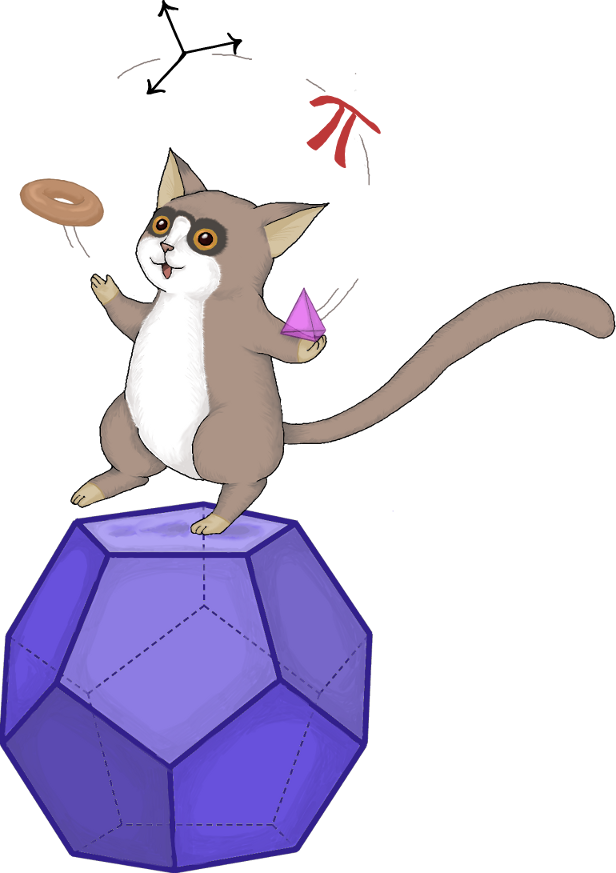
\includegraphics[scale=0.1]{../cover}}
}

\frame[plain]{\begin{center}
  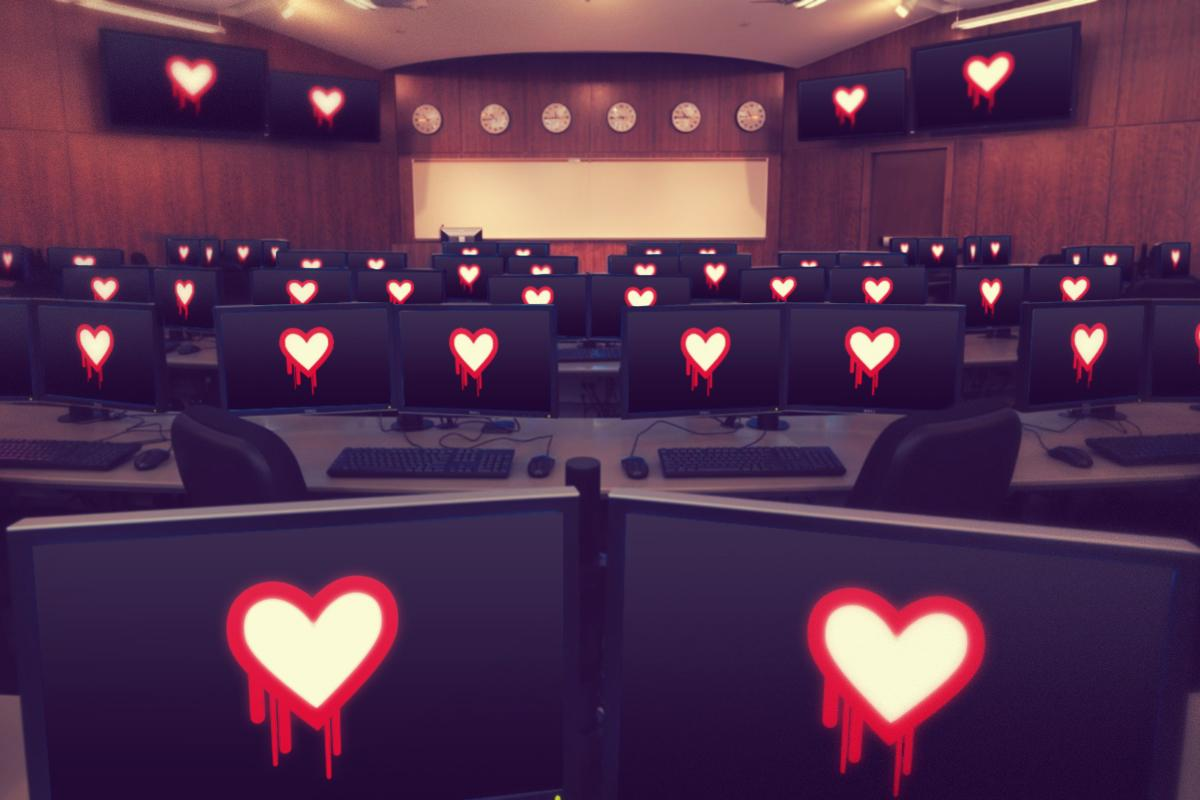
\includegraphics[scale=0.25]{images/heartbleed.jpeg}

  Der Heartbleed-Bug
\end{center}}

\section[Münzwurf]{Münzwurf über Telefon}
\frame[t]{\frametitle{Münzwurf über Telefon}
  \begin{itemize}
    \item
      Kontext: \\
      Alice und Bob telefonieren. \\
      Sie müssen entscheiden, welcher von ihnen eine unliebsame
      Aufgabe übernimmt.
      \floatbox{-70}{160}{
\includegraphics[scale=0.3]{images/coin-toss.png}}
  \end{itemize}
  \pause
  \vfill

  \begin{enumerate}
    \item Alice wählt Kopf, Bob wählt Zahl.
    \item Alice wirft eine Münze.
    \item Alice teilt Bob mit, dass die Münze Zahl anzeigt.
    \item Bob muss die Aufgabe übernehmen.
  \end{enumerate}
  \pause
  \vfill

  \begin{itemize}
    \item
      Offensichtlich: Alice kann betrügen!
  \end{itemize}
}

\frame[t]{\frametitle{Münzwurf über Telefon (Forts.)}
  \begin{itemize}
    \item
      Vereinfachung: \\
      Alice und Bob sitzen an einem Tisch. \\
      Sie müssen entscheiden, welcher von ihnen eine unliebsame
      Aufgabe übernimmt.
      \floatbox{-70}{160}{
\includegraphics[scale=0.3]{images/coin-toss.png}}
  \end{itemize}
  \pause
  \vfill

  \begin{enumerate}
    \item Alice nimmt eine Münze und legt sie unter eine Tasse.
          Bob weiß nicht, welche Seite nach oben zeigt.
    \item Bob entscheidet sich für Kopf oder Zahl.
    \item Alice deckt die Tasse auf.
  \end{enumerate}
  \pause
  \vfill

  \begin{itemize}
    \item Kein Zufall, Alice kontrolliert die Münze!
    \item Sicherheit durch gezwungene Festlegung
  \end{itemize}
}

\frame[t]{\frametitle{Einwegfunktionen}
  \begin{block}{Definition}
    Eine Rechenvorschrift~$H$ heißt genau dann \emph{Einwegfunktion},
    wenn es sehr schwierig ist, zu gegebenem
    Funktionswert~$y$ eine Stelle~$x$ mit
    $H(x) = y$
    zu finden.
  \end{block}
  \vfill

  \begin{tabbing}
    \quad\itembull\ \ \= kein Beispiel:\ \ \= Name \= $\longmapsto$ \= \kill
    \quad\itembull\ \ \> Beispiele: \> Name \> $\longmapsto$ \> Telefonnummer \\
                      \>            \> Text \> $\longmapsto$ \> SHA-256-Hash \\
    \quad\itembull\ \ \> kein Beispiel: \> Buch \> $\longmapsto$ \> ISBN \\\\
    \quad\itembull\ \ \> zusätzliche Forderung: Kollisionsresistenz
  \end{tabbing}
  \floatbox{-260}{5}{
\includegraphics[scale=0.09]{images/einweg.png}}
}

\frame[t]{\frametitle{Digitale Imitation (unsichere Variante)}
  \setbeamercovered{transparent}
  \begin{enumerate}
    \item Alice entscheidet sich für Kopf (oder Zahl): \\
          $M := \texttt{Münze zeigt Kopf}$
          \pause\vfill
    \item Alice berechnet eine Einwegfunktion und
          teilt Bob das Ergebnis mit: \\
          $H(M) = \texttt{698eb5c9bcb789548188db9cc4}$
          \pause\vfill
    \item Bob entscheidet sich für Kopf oder Zahl
          und teilt Alice seine Entscheidung mit.
          \pause\vfill
    \item Alice teilt Bob den Text~$M$ mit.
          \pause\vfill
    \item Bob berechnet seinerseits $H(M)$
          und überprüft so Alice' Ergebnis.
  \end{enumerate}
}

\frame[t]{\frametitle{Digitale Imitation (sichere Variante)}
  \setbeamercovered{transparent}
  \begin{enumerate}
    \item Alice entscheidet sich für Kopf (oder Zahl)
          und denkt sich ein Passwort aus: \\
          $M := \texttt{GeheimesPasswort, Münze zeigt Kopf}$
          \pause\vfill
    \item Alice berechnet eine Einwegfunktion und
          teilt Bob das Ergebnis mit: \\
          $H(M) = \texttt{ae30d422b3270dd66612c56637}$
          \pause\vfill
    \item Bob entscheidet sich für Kopf oder Zahl
          und teilt Alice seine Entscheidung mit.
          \pause\vfill
    \item Alice teilt Bob den Text~$M$ mit.
          \pause\vfill
    \item Bob berechnet seinerseits $H(M)$
          und überprüft so Alice' Ergebnis.
  \end{enumerate}
}

\section[D--H]{Diffie--Hellman-Schlüsselaustausch}
\frame[t]{\frametitle{Diffie--Hellman}
  \begin{itemize}
    \item Kontext: \\
	  Alice und Bob wollen ohne sonstige vorherige Absprachen ein
	  gemeinsames Geheimnis ausmachen.
  \end{itemize}

  \floatbox{-190}{135}{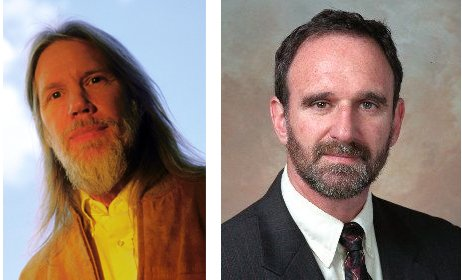
\includegraphics[scale=0.3]{images/diffie.jpeg}}
}

\frame[t]{\frametitle{Diffie--Hellman (Forts.)}
  \begin{changemargin}{-1em}{-1em}

  \begin{enumerate}
    \item Fest: $p$ Primzahl, $g$ Primitivwurzel modulo~$p$
    \item Alice und Bob erzeugen je eine Zufallszahl, $a$ bzw. $b$.
    \item Alice $\rightarrow$ Bob: \tabto{2.8cm}$A :\equiv g^a \mod p$ \\
          Bob $\rightarrow$ Alice: \tabto{2.8cm}$B :\equiv g^b \mod p$
    \item Alice und Bob berechnen das Geheimnis: \\
	  Alice: \tabto{1.3cm} $K :\equiv B^a \mod p$ \\
	  Bob:   \tabto{1.3cm} $K :\equiv A^b \mod p$
  \end{enumerate}
  \vfill

  \begin{itemize}
    \item Gleiche Ergebnisse~$K$!
    \item Worauf basiert die Sicherheit?
    \item Welche Schwachstelle hat das Verfahren?
  \end{itemize}
  \end{changemargin}
}

\section{Elliptische Kurven}
\frame[t]{\frametitle{Elliptische Kurven}
  \begin{itemize}
    \item {\small\url{http://en.wikipedia.org/wiki/Elliptic_curve}}
    \item Dank der Gruppenstruktur kann man Diffie--Hellman auch mit
    elliptischen Kurven durchführen. Vorteil: Kürzere Schlüssellängen möglich,
    spannende Mathematik.
    \item Außerdem kann man Pseudozufallszahlen erzeugen (Tafel).
    \item Vermutlich hat die NSA in eine bestimmte Variante eine Hintertür
    eingebaut (Tafel).
  \end{itemize}

  \floatbox{-260}{40}{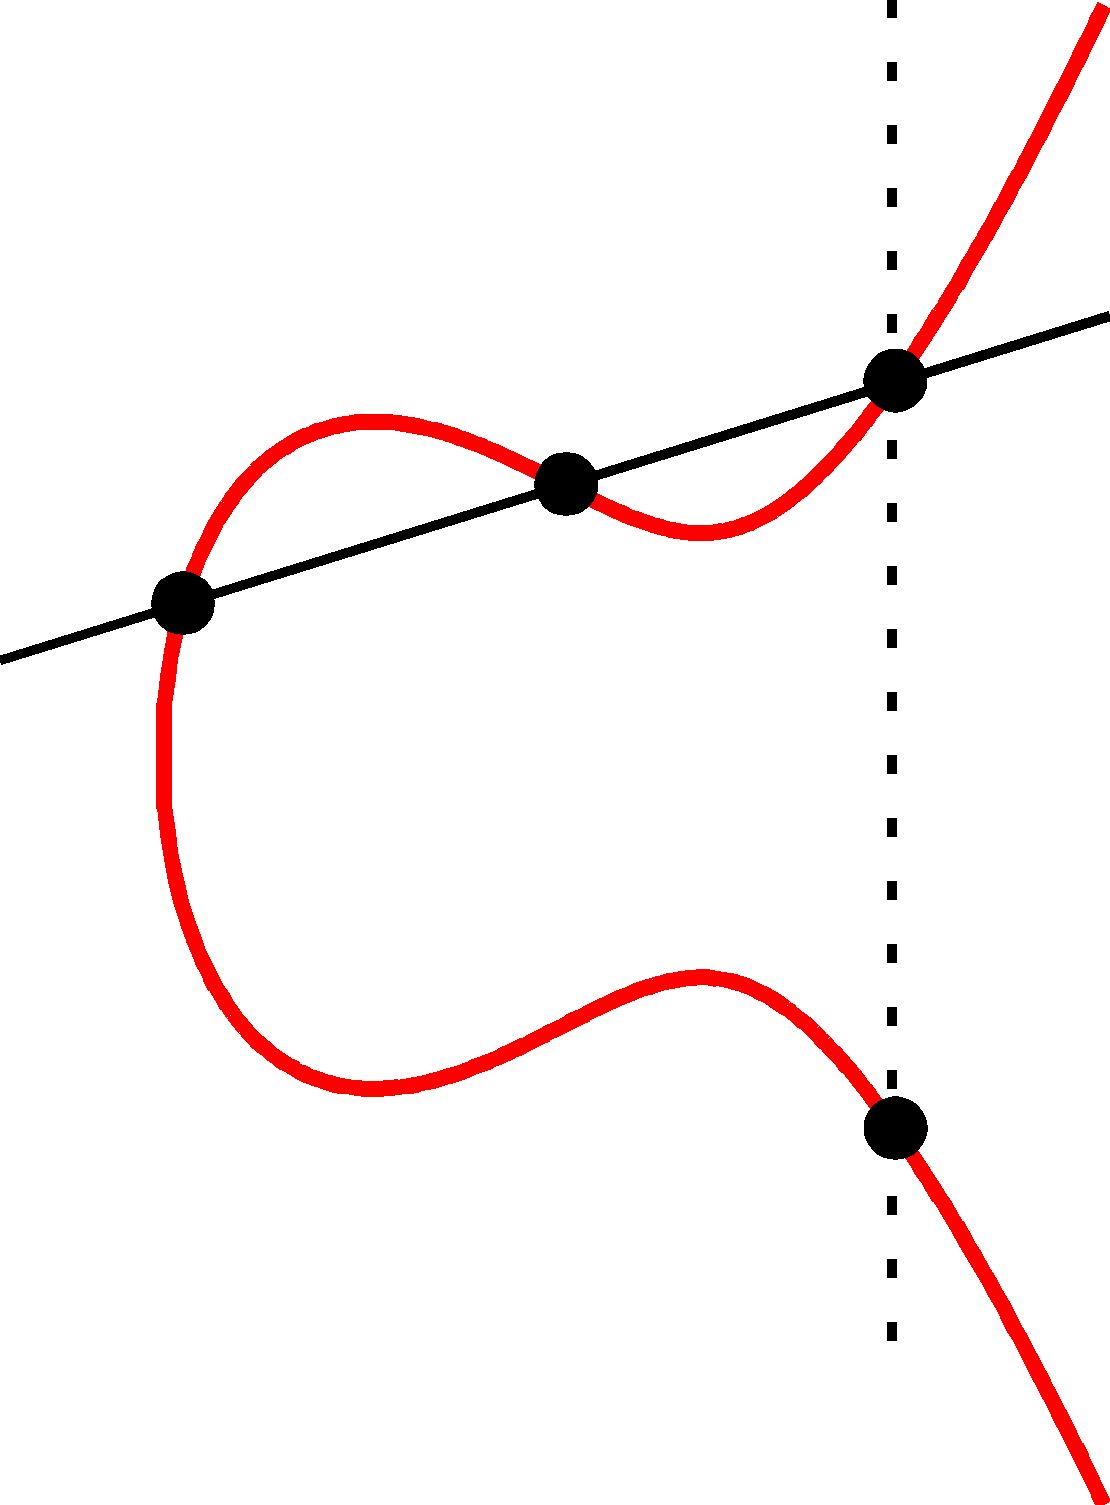
\includegraphics[scale=0.05]{images/elliptic-curve.png}}
}

\appendix

\frame[t]{\frametitle{Bildquellen}
  \tiny
  \begin{itemize}
    \item \url{http://biblioragazzi.files.wordpress.com/2008/04/reference.jpg}
    \item \url{http://i34.tinypic.com/51ptu0.jpg}
    \item \url{http://imgs.xkcd.com/comics/code_talkers.png}
    \item \url{http://one-time-pad.tripod.com/otp.jpg}
    \item \url{http://upload.wikimedia.org/wikipedia/commons/2/2b/Caesar3.svg}
    \item \url{http://www.bryx.de/wp-content/uploads/2008/09/800px-zeichen_220svg.png}
    \item \url{http://www.cellphones.ca/news/upload/2008/09/knowledge1.jpg}
    \item \url{http://www.digitaltrends.com/wp-content/uploads/2014/04/Heartbleed-bug.jpg}
    \item \url{http://www.gpuri.com/images/213/21325.jpg}
    \item \url{http://www.hirt-institut.de/de/Media/Shop/CategoryTextMedia/hirt_motiv_ihre_ziele.jpg}
    \item \url{http://www.hpl.hp.com/research/info_theory/images/curveplot.gif}
    \item \url{http://www.kveller.com/images/Article_images/wheres_waldo.jpg}
    \item \url{http://www.marketoracle.co.uk/images/coin-toss.jpg}
    \item \url{http://www.treachery.net/images/why_security_through_obscurity_isnt.jpg}
    \item \url{http://www.waleed-security.com/wp-content/uploads/2008/11/bruceab.jpg}
  \end{itemize}
}

\end{document}

\section[Nullwissen]{Zero-Knowledge-Beweise}
\frame[t]{\frametitle{Zero-Knowledge-Beweise}
  \begin{itemize}
    \item
      Kontext: \\
      Alice möchte Bob davon überzeugen, dass sie ein bestimmtes Geheimnis
      kennt, ohne das Geheimnis preiszugeben.
      \floatbox{-125}{150}{%
	\only<1>{
\includegraphics[scale=0.25]{images/knowledge.jpeg}}%
	\only<2>{\hspace{1.5cm}
\includegraphics[scale=0.05]{images/schneier.jpeg}}%
      }
    \item
      Illustration: Wo ist Waldo?

    \pause
    \vfill
    \item Variante: Alice und Bob möchten \\ überprüfen, ob sie beide dasselbe \\
    Geheimnis kennen, ohne es \\ preiszugeben.
  \end{itemize}
}

